\documentclass[tikz,border=3mm]{standalone}
\usetikzlibrary{decorations.markings,arrows.meta,bending,shapes.misc}
\tikzset{% 
    attach arrow/.style={
    decoration={
        markings,
         mark=at position 0 with {\pgfextra{%
         \pgfmathsetmacro{\tmpArrowTime}{\pgfkeysvalueof{/tikz/arc arrow/length}/(\pgfdecoratedpathlength)}%
         \xdef\tmpArrowTime{\tmpArrowTime}}},
        mark=at position {#1-3*\tmpArrowTime} with {\coordinate(@1);},
        mark=at position {#1-2*\tmpArrowTime} with {\coordinate(@2);},
        mark=at position {#1-1*\tmpArrowTime} with {\coordinate(@3);},
        mark=at position {#1+\tmpArrowTime/2} with {\coordinate(@4);
        \draw[-{Stealth[length=\pgfkeysvalueof{/tikz/arc arrow/length},bend]}] plot[smooth]
         coordinates {(@1) (@2) (@3) (@4)};},
        },
     postaction=decorate,
     },
     attach arrow/.default=0.5,
     arc arrow/.cd,length/.initial=2mm,
}
\begin{document}
% \begin{tikzpicture}
% \path[nodes={circle,minimum size=2.4em,font=\bfseries\sffamily}] 
%     node[ball color=blue] (L){--} 
%     (2.5,0) node[ball color=red] (R){+};
% \foreach \X in {0,...,7}
%  {\draw[very thick,attach arrow] (L) 
%  to[bend left={-70+\X*20},looseness=1.6] 
%  (R);}
% \foreach \X in {0,...,10}
%  {\draw[very thick,attach arrow/.list={1/3,2/3}] (L) to[bend left=16-4*\X] ++ (70+\X*22:3);
%  \draw[very thick,attach arrow/.list={1/3,2/3}] (R)+(180+70+\X*22:3) 
%  to[bend right=16-4*\X] 
%   (R);}
% \end{tikzpicture}

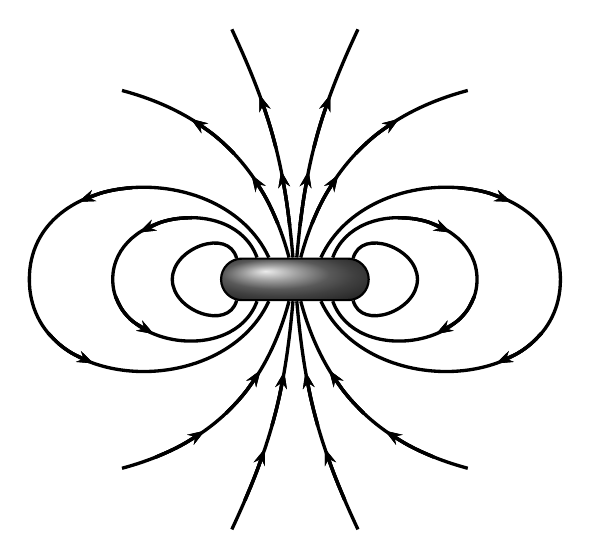
\begin{tikzpicture}[very thick, node distance = 2cm, auto,rotate=90,transform shape]
 \node[rounded rectangle,ball color=gray,draw,minimum width=6em,minimum
 height=1.5em,rotate=90,thick] (D){};
 \foreach \X in {2,...,4}
 {\draw[looseness=1.2] \ifnum\X<3
 \else [attach arrow/.list={1/3,2/3}] \fi (D.00-10*\X) to[out=5*\X+5,in=0] 
 ([yshift=\X*\X*1ex]D.east) to[out=180,in=180-5*\X-5] (D.00+10*\X);
 \draw[looseness=1.2] \ifnum\X<3
 \else [attach arrow/.list={1/3,2/3}] \fi 
 (D.180+10*\X) to[out=-5*\X-5,in=0]  ([yshift=-\X*\X*1ex]D.west)
 to[out=180,in=180+5*\X+5] (D.180-10*\X);}
 \foreach \X in {0,...,3}
 {\draw[attach arrow/.list={1/3,2/3}] (D.-90+15-10*\X) to[bend
 right=30-20*\X] ++ (45-30*\X:3);
 \draw[attach arrow/.list={1/3,2/3}] (D.90+15-10*\X) 
  ++ (225-30*\X:3) to[bend left=30-20*\X] (D.90+15-10*\X);
 }
\end{tikzpicture}
\end{document}
